\documentclass[conference]{IEEEtran}
\IEEEoverridecommandlockouts
% The preceding line is only needed to identify funding in the first footnote. If that is unneeded, please comment it out.
\usepackage{cite}
\usepackage{amsmath,amssymb,amsfonts}
\usepackage{algorithmic}
\usepackage{graphicx}
\usepackage{textcomp}
\usepackage{xcolor}
\def\BibTeX{{\rm B\kern-.05em{\sc i\kern-.025em b}\kern-.08em
    T\kern-.1667em\lower.7ex\hbox{E}\kern-.125emX}}
    
\usepackage{listings}
\usepackage{xcolor}

\usepackage{hyperref}

%New colors defined below
\definecolor{codegreen}{rgb}{0,0.6,0}
\definecolor{codegray}{rgb}{0.5,0.5,0.5}
\definecolor{codepurple}{rgb}{0.58,0,0.82}
\definecolor{backcolour}{rgb}{0.95,0.95,0.92}

%Code listing style named "mystyle"
\lstdefinestyle{mystyle}{
  backgroundcolor=\color{backcolour},   commentstyle=\color{codegreen},
  keywordstyle=\color{magenta},
  numberstyle=\tiny\color{codegray},
  stringstyle=\color{codepurple},
  basicstyle=\ttfamily\footnotesize,
  breakatwhitespace=false,         
  breaklines=true,                 
  captionpos=b,                    
  keepspaces=true,                 
  numbers=left,                    
  numbersep=5pt,                  
  showspaces=false,                
  showstringspaces=false,
  showtabs=false,                  
  tabsize=2
}

%"mystyle" code listing set
\lstset{style=mystyle}
    
\begin{document}

\title{ECE 575 Final Project: Implementing a 5-stage processor pipeline in Python}

\author{\IEEEauthorblockN{Robert Werthman}
\IEEEauthorblockA{ECE 575 Section 02 \\
University of Michigan Dearborn}
}

\maketitle

\begin{abstract}
This document describes an implementation of a 5-stage instruction processing pipeline in the programming language Python.  The processor, pipeline stages, instructions, and data memory can be represented in Python using object-oriented programming and python structures like lists and dictionaries.  The pipeline is based on the MIPS pipeline describe in [1, p. 301]
\end{abstract}

\section{Introduction}
There are multiple ways to execute instructions in a processor.  One way is to execute one instruction in one clock cycle.  This is known as single cycle execution.  In single cycle execution the processor datapath, all the elements necessary to implement a set of instructions, is designed such that all instructions that are part of the instruction set architecture are executed in a single clock cycle [2, p. 1].  An often used analogy to the execution of an instruction is doing laundry as mentioned in [1, p. 272].  Let's say the instruction you wanted to execute was to wash dirty cloths and put them away.  In a single cycle datapath the steps would be
\begin{enumerate}
    \item Put dirty cloths in washer.
    \item Once washer is done put dirty cloths in dryer.
    \item When dryer is done put clothes away.
\end{enumerate}
As you can see each step depends on the completion of the previous step.  Imagine you had a roommate who was doing laundry after you. The roommate would have to wait for your load of laundry to be done before starting their load of laundry.  If you and your roommate did laundry according to single cycle datapath, you would do your load of laundry in the first cycle and your roommate would do their laundry in the second cycle.  As it turns out this is not a very efficient to execute instructions--or do laundry.  A better way is called the pipelined datapath.

An instruction is a series of steps.  All steps need to be completed in order for the instruction to be completed.  In a pipelined datapath one step of an instruction is executed in a clock cycle.  This is contrary to the single cycle datapath where all of the steps of an instruction are executed in a clock cycle.  Using the clothes washing analogy again, the steps in a pipelined datapath would be
\begin{enumerate}
    \item Put dirty cloths in washer.
    \item Once washer is done put dirty cloths in dryer.  Roommate puts dirty clothes in washer.
    \item Once dryer is done put clothes away.  Roommate puts clothes from washer into dryer.
    \item Roommate puts clothes away.
\end{enumerate}
You may have noticed the roommate does not have to wait for your clothes to be completely done before starting their laundry.  The roommate can use the washer as long as you don't have any clothes in it.  This ends up being a more efficient design for a processor datapath than the single cycle.
As noted in [1, pp. 286] the steps of an instruction in a pipelined datapath are broken up into 5-stages
\begin{enumerate}
\item IF: Instruction fetch
\item ID: Instruction decode and register file read
\item EX: Execution or address calculation
\item MEM: Data memory access
\item WB: Write Back
\end{enumerate}
These stages can be modelled in Python as objects connected to each other.  The rest of this document describes the implementation of this model.

\section{Architecture}

\begin{figure}
    \centering
    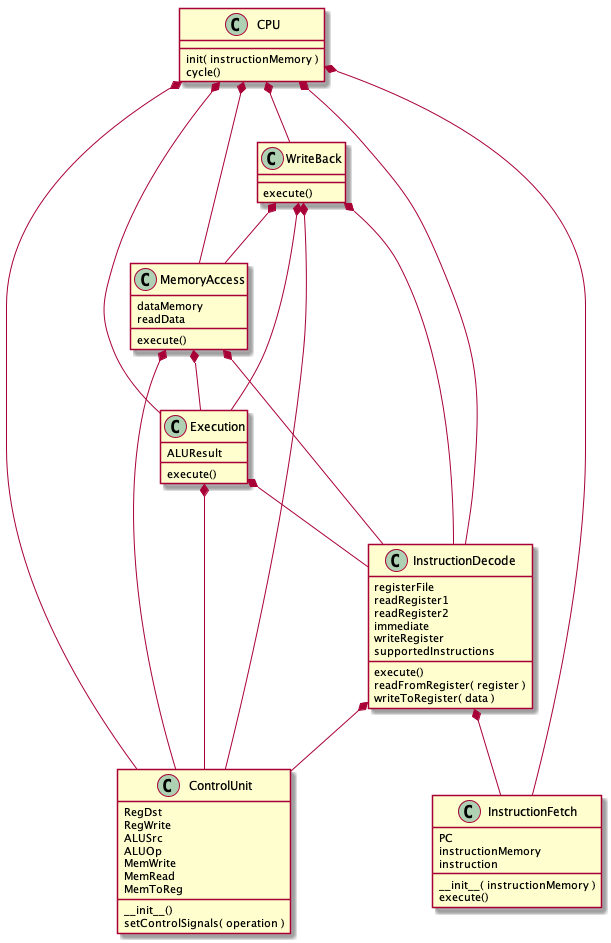
\includegraphics[scale=.4]{architecture.png}
    \caption{Class Diagram of Python Implementation}
    \label{fig:class_diagram}
\end{figure}

The Python implementation is made of the 5 pipeline stages mentioned in the introduction.  These are represented as Python classes.  Each of these stages consist of additional components like
\begin{itemize}
    \item instruction memory
    \item data memory
    \item a register file
    \item an ALU (arithmetic logic unit)
    \item a PC (program counter)
    \item a control unit
\end{itemize}
All of these components belong to different stages of the pipeline except for the control unit which is used in almost all stages of the pipeline.  A class diagram of the architecture can be seen in figure \ref{fig:class_diagram}.

The current architecture only supports a limited number of r-type and i-type instructions.  Branch instructions are not currently supported.

\subsection{IF: Instruction Fetch}

\begin{figure}
    \centering
    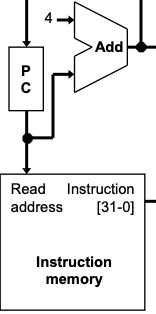
\includegraphics[scale=.4]{instructionfetch.png}
    \caption{Instruction Fetch Stage [2]}
    \label{fig:instructionfetch}
\end{figure}

The instruction fetch part of the pipeline takes the program counter (PC) and fetches the instruction at the address of the program counter [1, pp. 300].  It increments the program counter to the next address.  These things are done in a class method called execute which all stages of the pipeline have.  Figure \ref{fig:instructionfetch} depicts the components of the instruction fetch stage.

\subsubsection{Instruction Memory}

Instruction memory is represented as a Python list that is passed into the instruction fetch class at initialization.  Each instruction itself is also a Python list.  Depending on the instruction type the list is made up of the opcode, source and destination registers, address/immediate value, etc.  An example of an add instruction in python 

\begin{lstlisting}[language=Python]
# An add instruction
instruction = [ "add", "r1", "r2", "r3" ]
\end{lstlisting}

which means [3, pp. 194]

\begin{center}
\begin{tabular}{|c|c|c|c|}
\hline
     op & rs & rt & rd \\
\hline
\end{tabular}
\end{center}

To access the instruction memory you use an index into the instruction memory list.  For example
\begin{lstlisting}[language=Python]
# Get the first instruction from instruction memory
instruction = instructionMemory[0]
\end{lstlisting}

\subsubsection{Program Counter}

The program counter is a python variable that is initialized as 0 and is increment by 1 for every call to the execute method of the instruction fetch class.  The program counter cannot exceed the size of the instruction memory list.

\subsection{ID: Instruction Decode}

\begin{figure}
    \centering
    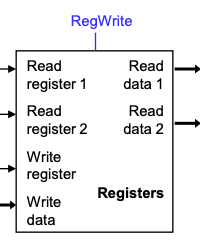
\includegraphics[scale=.4]{instructiondecode.png}
    \caption{Instruction Decode Stage [2]}
    \label{fig:instructiondecode}
\end{figure}

The instruction decode stage gets the instruction from the instruction fetch stage through a class instance member variable.  The control signals for the instruction are set in the control unit based on the opcode in the instruction.  The read registers, rs and rt, are stored in the instruction decode class as well as the write register, and the immediate/address value if one exists.  These come from the instruction retrieved in the instruction fetch stage.  Only add, load word (lw), and store word (sw) are supported instructions at this time.  The supported instructions are mapped to their instruction type in a dictionary.

\begin{lstlisting}[language=Python]
self.supportedInstrutions = {
            "add" : "rtype",
            "lw"  : "itype",
            "sw"  : "itype"
        }
\end{lstlisting}

The instruction type is used to determine if there will be an immediate/address in the instruction or not. 
There are 2 methods that are a part of the instruction decode stage.  They are the readFromRegister and writeToRegister methods similiar to the read data and write data in [1, pp. 301].
The instruction decode stage has a register file.  The components of the instruction decode phase can be seen in \ref{fig:instructiondecode}.

\subsubsection{Register File}

The register file is a dictionary with the register as the key and value of the register as the value.

\begin{lstlisting}[language=Python]
self.registerFile = {
            "r1" : 2,
            "r2" : 1,
            "r3" : 0
        }
\end{lstlisting}
Only 3 registers are supported at this time.

\subsubsection{Control Unit}

\begin{figure}
    \centering
    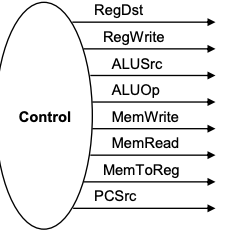
\includegraphics[scale=.4]{controlunit.png}
    \caption{Datapath Control Unit}
    \label{fig:controlunit}
\end{figure}

The control unit is a class that contains just member variables which are the control signals used in the different stages of the pipeline.  The signals are set to their proper values depending on what the opcode of the instruction is.  The control unit is seen in figure \ref{fig:controlunit}

\subsection{EX: Execution}

\begin{figure}
    \centering
    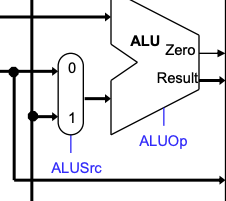
\includegraphics[scale=.4]{execution.png}
    \caption{Execution Stage}
    \label{fig:execution}
\end{figure}

In the execution state of the pipeline we compute the result of an arithmetic operation between 2 registers, or compute an address to load or store a value in data memory.  The execution stage depends on control signal ALUOp to tell it what type of arithmetic operation to perform.  It also depends on ALUSrc to tell it what should be the source of the second ALU operand.  The execution stage is seen in figure \ref{fig:execution}  Right now only the add ALU operation is supported.  This allows for an add r-type instruction or the load word or store word i-type instructions.

The result of the arithmetic operation is stored as a class instance member variable that both the Memory Access and Write Back stages will use.

\subsection{MEM: Memory Access}

In the memory access stage you can read or write data to/from data memory.  Depending on the instruction you may not use the memory access stage at all like in the case of an r-type instruction.  This stage is comprised of the data memory and the ability to use an address to read and write data.  The memory access stage is depicted in \ref{fig:memoryaccess}.

\subsubsection{Data Memory}

\begin{figure}
    \centering
    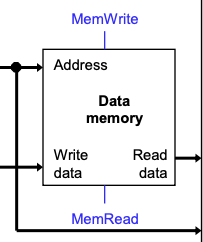
\includegraphics[scale=.4]{memoryaccess.png}
    \caption{Memory Access Stage [2]}
    \label{fig:memoryaccess}
\end{figure}

Much like the instruction memory, data memory is represented as a list of integers.  The address into data memory is the index of the item in the list you want to read or write.

\begin{lstlisting}[language=Python]
# Data memory
dataMemory = [1, 2, 3, 4]

# Data from first address in data memory
data = dataMemory[0]
\end{lstlisting}

The ALUResult that comes from the Execution stage is used as an index into the data memory list.  Depending on the values of the control signals MemRead or MemWrite you will either be reading or writing to the data memory.  An if/else statement is used with these control signals to determine if instruction is to read or write to data memory.

\subsection{WB: Write Back}

\begin{figure}
    \centering
    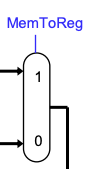
\includegraphics[scale=.4]{writeback.png}
    \caption{Write Back Stage [2]}
    \label{fig:writeback}
\end{figure}

The Write Back is the simplest of all of the stages, but it is the stage that depends the most on the previous stages.  As depicted in [1, pp. 301] and \ref{fig:writeback} this stage has a multiplexer (MUX) that is controlled by the MemToReg control signal.  The value of this signal depends on the instruction being executed.  The MUX is represented by an if/else statement with the MemToReg as the if condition.

\begin{lstlisting}[language=Python]
if controlUnit.MemToReg:
    ID.writeToRegister( MEM.readData )
else:
    ID.writeToRegister( EX.ALUResult )
\end{lstlisting}

\subsection{CPU}
The CPU is the main class that creates and contains all of the pipeline stages.  It is the class that initializes the instruction memory, passes it to the instruction fetch stage, and starts the execution of the pipeline.

The the execution of the stages is done in a method called \textit{cycle}.  This cycle method simulates a clock cycle and for each instruction in instruction memory execute the pipeline stages in order.

\begin{lstlisting}[language=Python]
for instruction in instructionMemory:
    IF.execute()
    ID.execute()
    EX.execute()
    MEM.execute()
    WB.execute()
\end{lstlisting}

Once all of the instructions are executed the program ends.

\section{Testing and Verification}

Test driven development was used when developing this project.  This means tests were written, the tests failed, and then code was written to make the tests pass.  For each class, a python file containing containing tests was created.  These tests were used to verify the behavior of each of the methods of the class.
The main driver of verification was the integration tests for the CPU.  In those tests a CPU was created that contained all of the stages of the pipeline and an instruction memory with one instruction.  The CPU processed the instruction through all of the pipeline stages.  At the end of the test, either data memory or a register was checked to see if it contained the right value in the right place.
\begin{lstlisting}[language=Python]
# $r1 = Memory[$r3 + 2]
instructionMemory = [
    [
        "sw", # op
        "r3", # rs
        "r1", # rt
        2 # address
    ]
]
cpu = CPU( instructionMemory )
cpu.cycle()
self.assertEqual( cpu.MEM.dataMemory[2], 2 )
\end{lstlisting}

The next step for testing is to have an instruction memory with multiple instructions to further verify the behavior of the code.

\section{Open Issues And Future Work}

\subsection{Open Issues}

The implementation doesn't currently support all instruction types nor does it support all instructions within the types it does support.  It has a very small amount of memory data, instruction data, and a tiny register file.  As was mentioned in the testing section, the testing has been limited and should be expanded to cover multi instruction instruction memory.

\subsection{Future Work}

The implementation is not exactly a pipelined implementation.  Only one instruction is run at a time through all of the stages.  This is more like a single cycle datapath.  In order for it to be a correct pipeline implementation the values shared between each pipeline stage would need an in and out holding area.  This area would be similar to a double buffer in computer graphics.  One buffer would have the current value being used, the other buffer would contain the value to be used next.  If you look at figure \ref{fig:pipeline_double_buffer}, the column with the red rectangle represents this idea of a double buffer.

Let's say you have an instruction memory with 2 instructions.  For the instruction fetch stage on the first clock cycle, instruction 1 would passed to the \textbf{in} buffer of the instruction decode phase.  On the next cycle it would be passed to the \textbf{out} buffer of the instruction decode phase.  Instruction 2 would also be put in the \textbf{in} buffer of the instruction decode phase.  Once something is in the \textbf{out} buffer it can be used in that stage.  This means in the second cycle, instruction 1 is put into the out buffer and instruction decode stage is run on this instruction.  This is depicted in figure \ref{fig:double_buffer}.

\begin{figure}
    \centering
    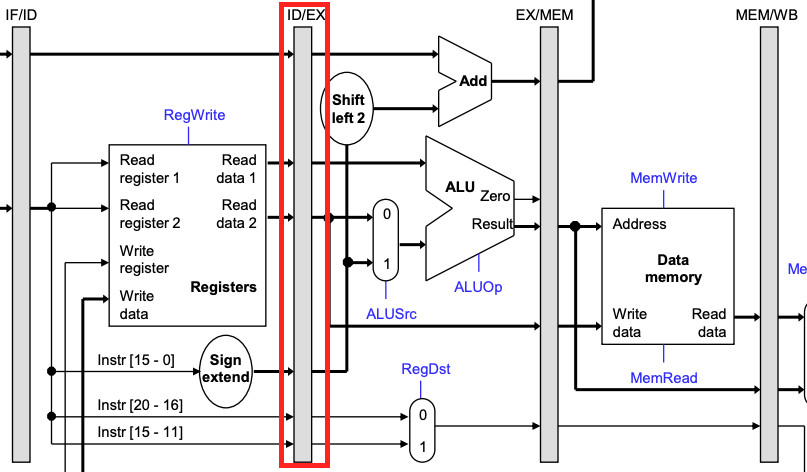
\includegraphics[scale=.3]{pipeline_double_buffer.png}
    \caption{Pipeline Double Buffer [2]}
    \label{fig:pipeline_double_buffer}
\end{figure}

\begin{figure}
    \centering
    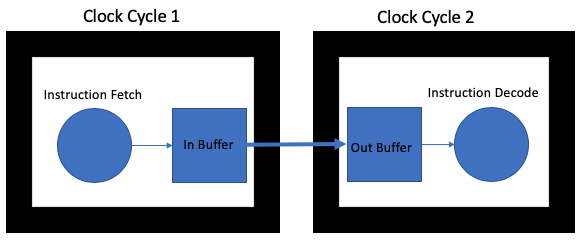
\includegraphics[scale=.3]{double_buffer.png}
    \caption{Double Buffer}
    \label{fig:double_buffer}
\end{figure}

\begin{thebibliography}{00}
\bibitem{b1} J. Hennessy and D. Patterson, \textit{Computer Organization And Design: The Hardware/Software Interface}, 5th ed. Waltham, MA: Elsevier, 2014.
\bibitem{b2} L. Ceze, "A single-cycle MIPS processor". University of Washington, Computer Science and Engineering, CSE 378, Winter 2009. [Online]. Available: \url{https://courses.cs.washington.edu/courses/cse378/09wi/lectures/lec07.pdf}. [Accessed December 03, 2019]
\bibitem{b3} P. Gillard, "The MIPS instruction set architecture". Memorial University, Department of Computer Science, CS 3725. [Online]. Available: \url{http://web.cs.mun.ca/~paul/cs3725/material/review.pdf}. [Accessed December 03, 2019]
\end{thebibliography}

\end{document}
